%%%% Header %%%%%%%%%%%%%%%%%%%%%%%%%%%%%%%%%%%%%%%%%%%%%%%%%%%%%%%%%%%%%%%%%%%

\documentclass{beamer}

\usepackage{jobeam}

\bibliography{/home/jon/lucile/share/jowncloud/sci/refs/refs.bib}
\hyphenation{}

%%%% Meta Data %%%%%%%%%%%%%%%%%%%%%%%%%%%%%%%%%%%%%%%%%%%%%%%%%%%%%%%%%%%%%%%%

\title{The Gestational Age Pattern\\of Human Mortality}
\author{Jonas Schöley\\\url{jschoeley@health.sdu.dk}}

%%%% Titlepage %%%%%%%%%%%%%%%%%%%%%%%%%%%%%%%%%%%%%%%%%%%%%%%%%%%%%%%%%%%%%%%%

\begin{document}

{
\begin{frame}[plain]
\titlepage
\end{frame}
}

\clearpage

\section{Explaining Ontogenescence} %%%%%%%%%%%%%%%%%%%%%%%%%%%%%%%%%%%%%%%%%%%

\begin{frame}
\frametitle{\insertsection}

2 Levels of Explanation:

\begin{itemize}
\item \emph{Individual}: The mortality decline over age represents growth, acquired robustness, adaptation to surroundings, risk mitigation taking place within an organism.
\item \emph{Population}: The mortality decline over age represents a selection effect: On average, the frailest individuals die first, the stronger individuals survive. Therefore, on the population level, the mean risk of death decreases over age.
\end{itemize}

\end{frame}

\begin{frame}
\frametitle{\insertsection}

\begin{figure}[htb!]
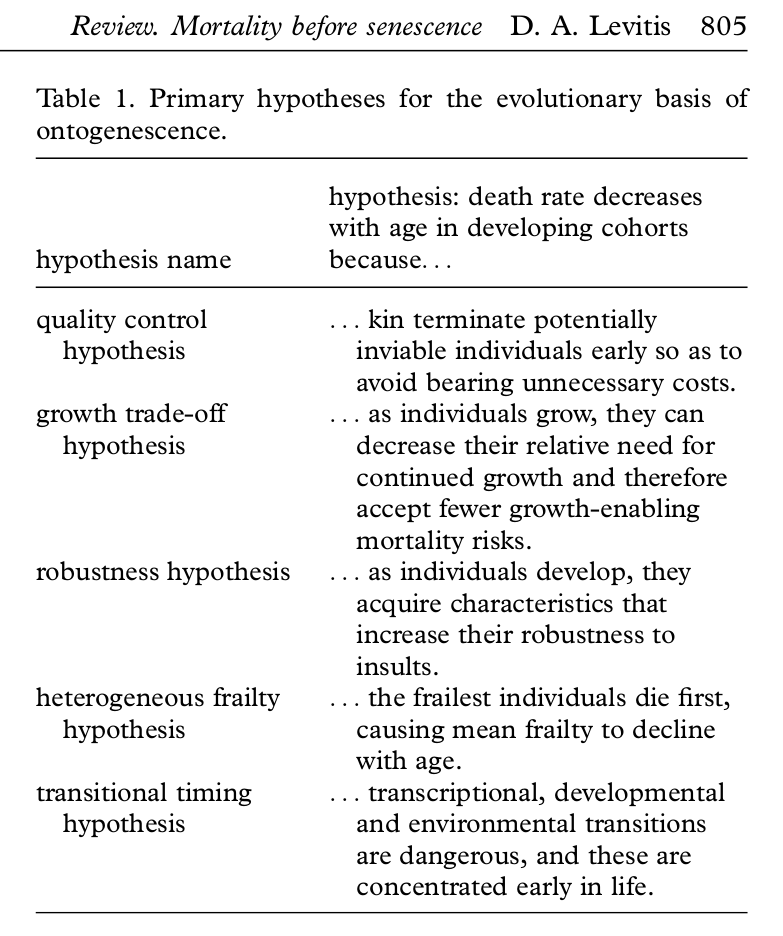
\includegraphics[width = 0.6\textwidth]{./fig/danielle_hypotheses.png} \\
\cite{Levitis2011}
\end{figure}

\end{frame}

\section{The Age Pattern of Infant Mortality} %%%%%%%%%%%%%%%%%%%%%%%%%%%%%%%%%

\begin{frame}
\frametitle{\insertsection}

\begin{figure}[htb!]
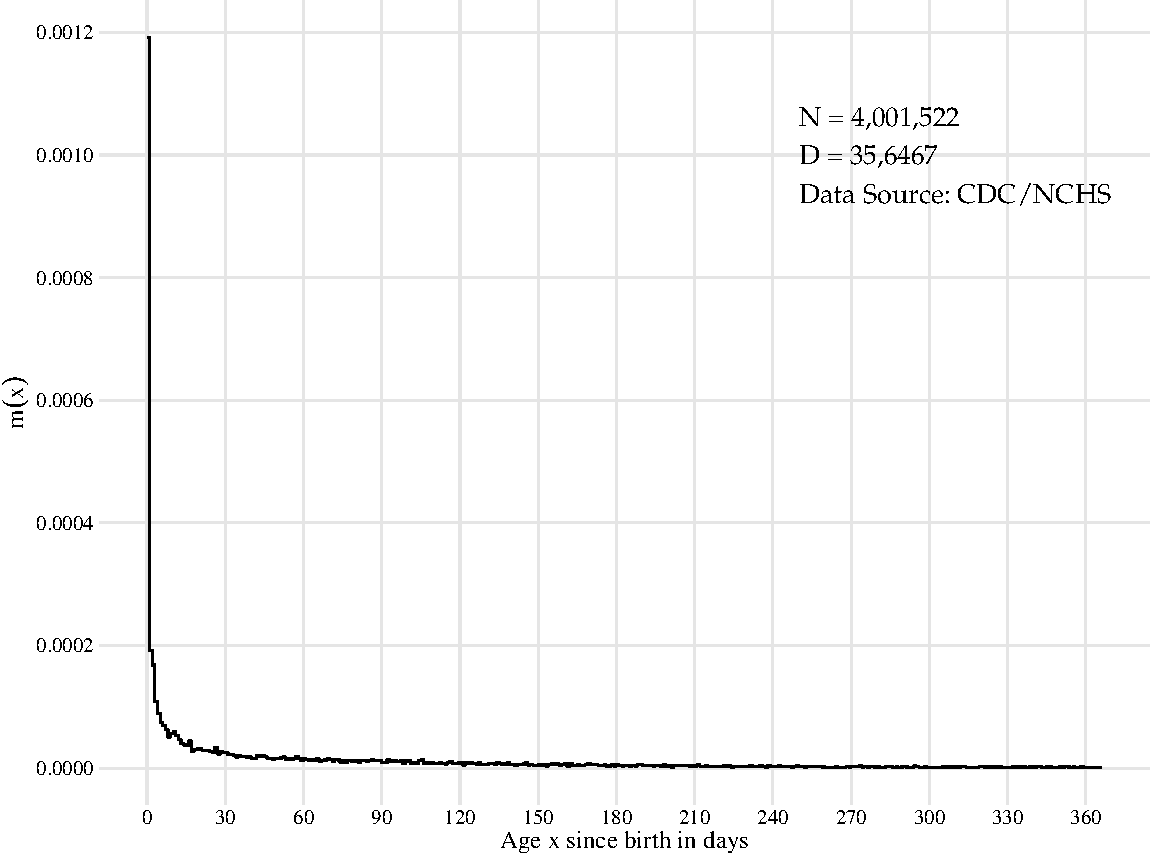
\includegraphics[width = 0.9\textwidth]{./fig/imort_mx.pdf} \\
The daily age pattern of infant mortality, US, conception cohort 2009.
\end{figure}

\end{frame}

\begin{frame}
\frametitle{\insertsection}

\begin{figure}[htb!]
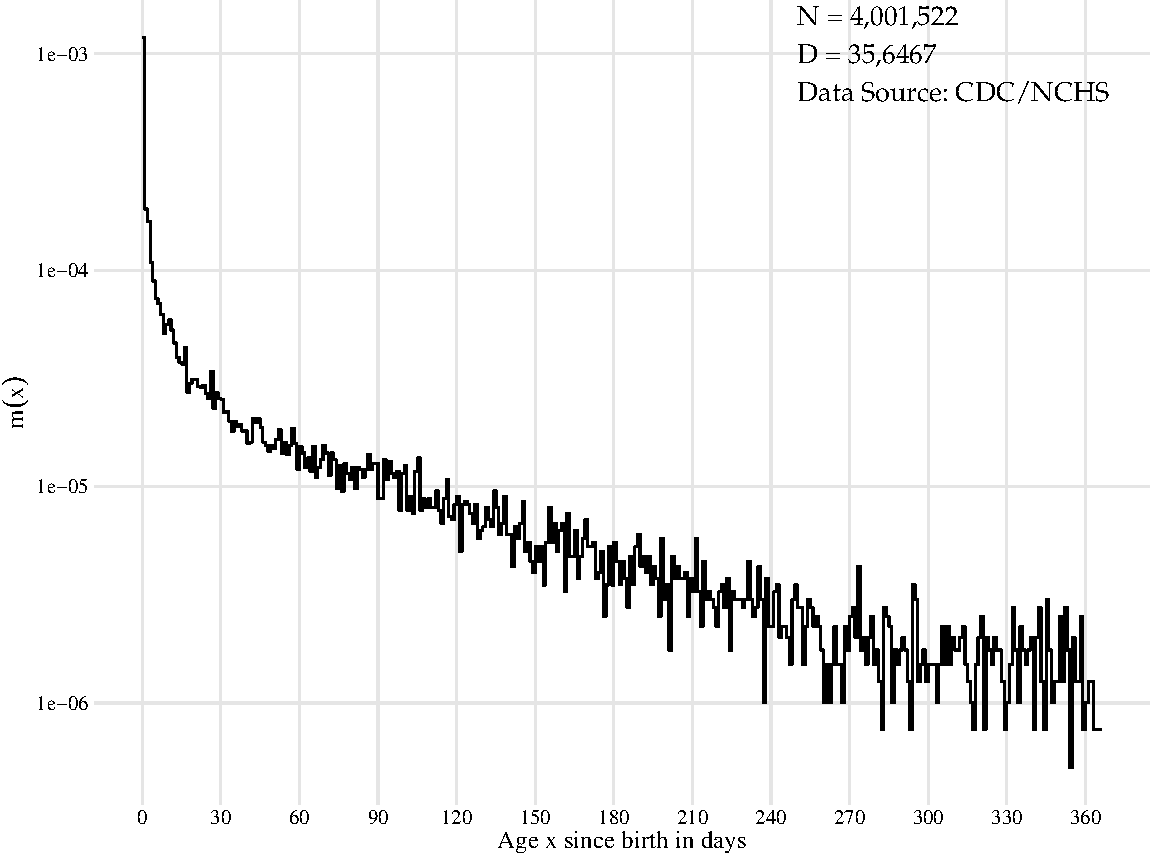
\includegraphics[width = 0.9\textwidth]{./fig/imort_log_mx.pdf} \\
The daily age pattern of infant mortality, log-mortality scale, US, conception cohort 2009.
\end{figure}

\end{frame}

\section{The Shape of Adaptation} %%%%%%%%%%%%%%%%%%%%%%%%%%%%%%%%%%%%%%%%%%%%%

\begin{frame}
\frametitle{\insertsection}

\small{\emph{Assumption}: The age pattern of adaptation is inverse to the age pattern of growth level (and should therefore be negative exponential).}

\begin{figure}[htb!]
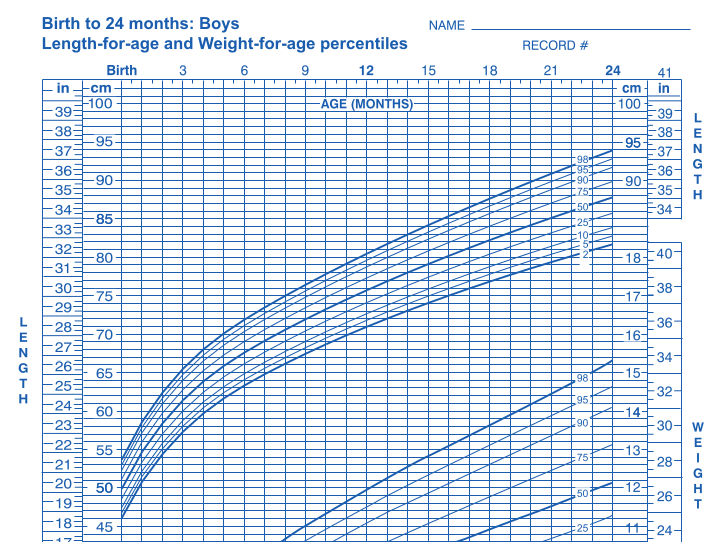
\includegraphics[width = 0.75\textwidth]{./fig/igrowth.png} \\
Average growth levels of infants over weeks after birth. \cite{WHO2009}.
\end{figure}

\end{frame}

\section{The Three Components of Infant Mortality} %%%%%%%%%%%%%%%%%%%%%%%%%%%%

\begin{frame}
\frametitle{\insertsection}

\begin{enumerate}
\item Mortality outlier at day of birth explained by \emph{transitional timing}
\item Exponential decrease of mortality after 50 days of age explained by \emph{adaptation}
\item Super exponential decrease of mortality right after birth explained by \emph{selection} of the least frail
\end{enumerate}

\end{frame}

\section{The Gestational Age Transformation \ldots} %%%%%%%%%%%%%%%%%%%%%%%%%%%

\begin{frame}
\frametitle{\insertsection}

\begin{columns}[c]

\column{0.33\textwidth}

\begin{figure}[htb!]
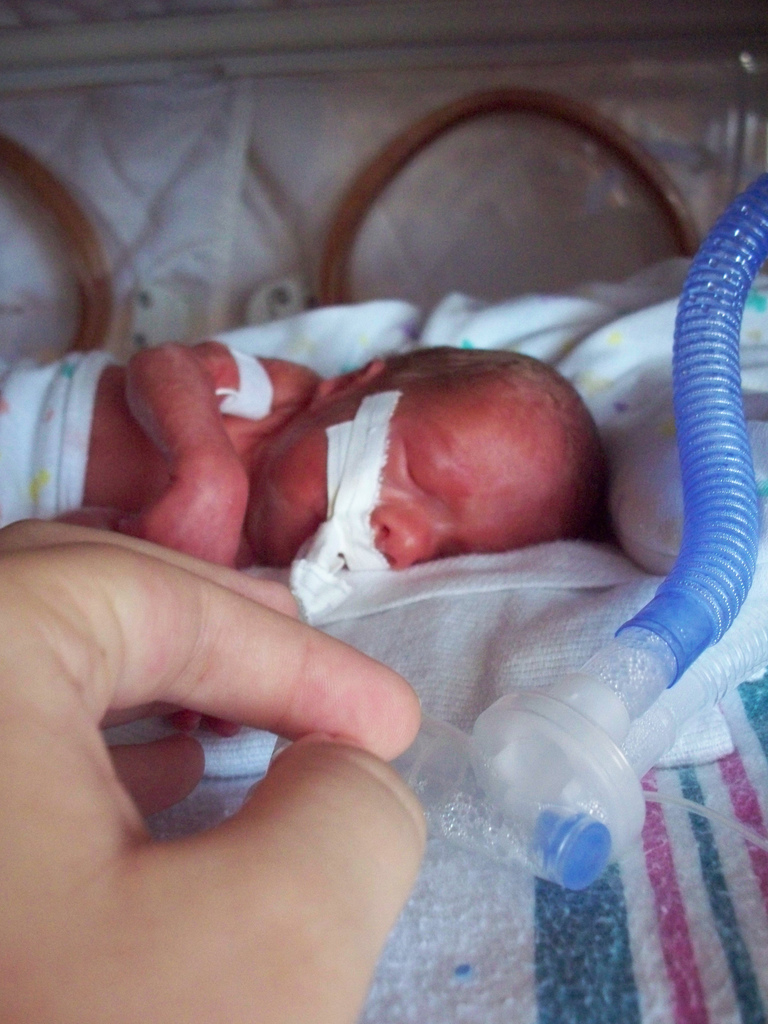
\includegraphics[]{./fig/premature_newborn.jpg} \\
Newborn, gestational age 26 weeks.
\end{figure}

\column{0.67\textwidth}
\begin{figure}[htb!]
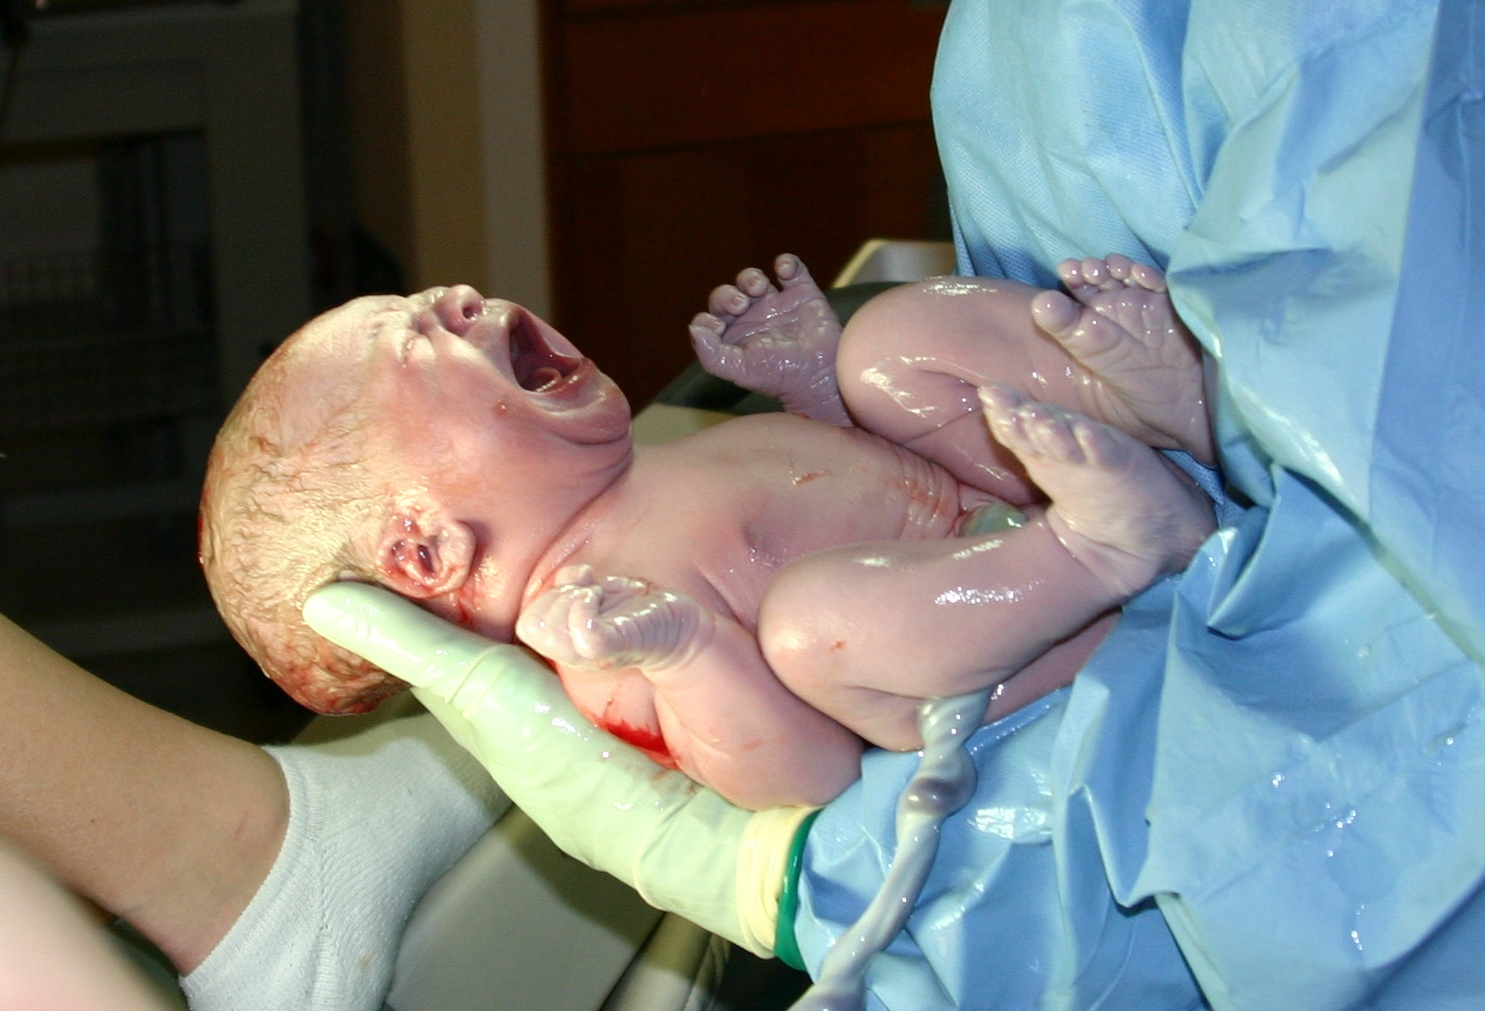
\includegraphics[]{./fig/newborn.jpg} \\
Newborn, gestational age about 40 weeks.
\end{figure}

\end{columns}

\end{frame}

\begin{frame}
\frametitle{\insertsection}

\begin{itemize}
\item \ldots de-clusters the event of birth
\item \ldots eliminates \emph{all} unobserved heterogeneity resulting from different gestational ages at birth
\end{itemize}

\end{frame}

\begin{frame}
\frametitle{\insertsection}

\begin{figure}[htb!]
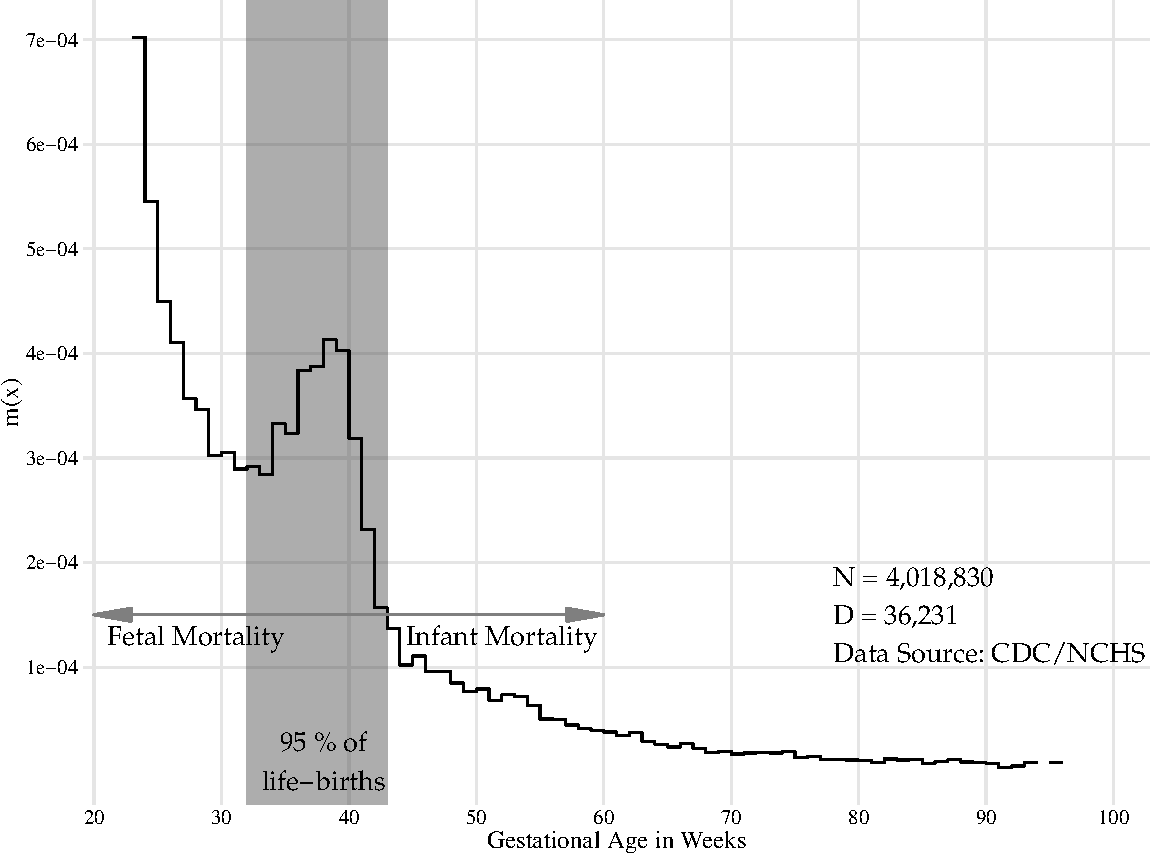
\includegraphics[width = 0.9\textwidth]{./fig/fimort_mx.pdf} \\
The gestational age pattern of human mortality, US, conception cohort 2009.
\end{figure}

\end{frame}

\begin{frame}
\frametitle{\insertsection}

\begin{figure}[htb!]
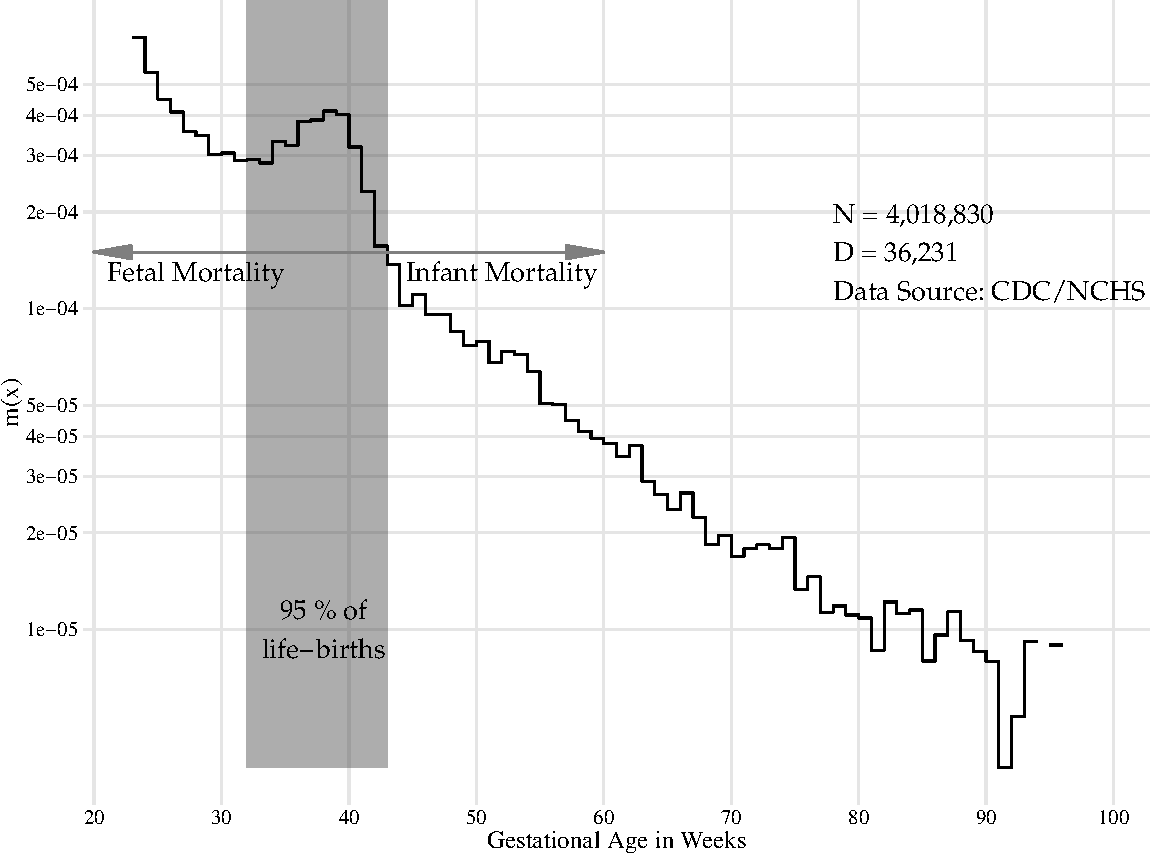
\includegraphics[width = 0.9\textwidth]{./fig/fimort_log_mx.pdf} \\
The gestational age pattern of human mortality, US, conception cohort 2009.
\end{figure}

\end{frame}

\section{The Model} %%%%%%%%%%%%%%%%%%%%%%%%%%%%%%%%%%%%%%%%%%%%%%%%%%%%%%%%%%%

\begin{frame}
\frametitle{\insertsection}

\begin{enumerate}
\item Mortality outlier at day of birth explained by \emph{transitional timing}
\item Exponential decrease of mortality after 50 days of age explained by \emph{adaptation}
\item Super exponential decrease of mortality right after birth explained by \emph{selection} of the least frail
\end{enumerate}

\end{frame}

\begin{frame}
\frametitle{\insertsection}

\begin{enumerate}
\item $\alpha_1 F(b)$: A factor representing the increased mortality risk in the perinatal period, weighted by the distribution of gestational ages at onset of labour
\item $\alpha_2 \text{e}^{\lambda x}$: A negative exponential function representing individual level adaptation and acquired robustness with age
\item $Z(x)$: A distribution of frailties at age $x$
\end{enumerate}

$$
m(x) = \alpha_1 F(b) + Z(x) \cdot \alpha_2 \text{e}^{\lambda x}
$$

\end{frame}

\begin{frame}
\frametitle{\insertsection}

$\text{f}(b)$ empirical, e.g. taken from data.

\begin{figure}[htb!]
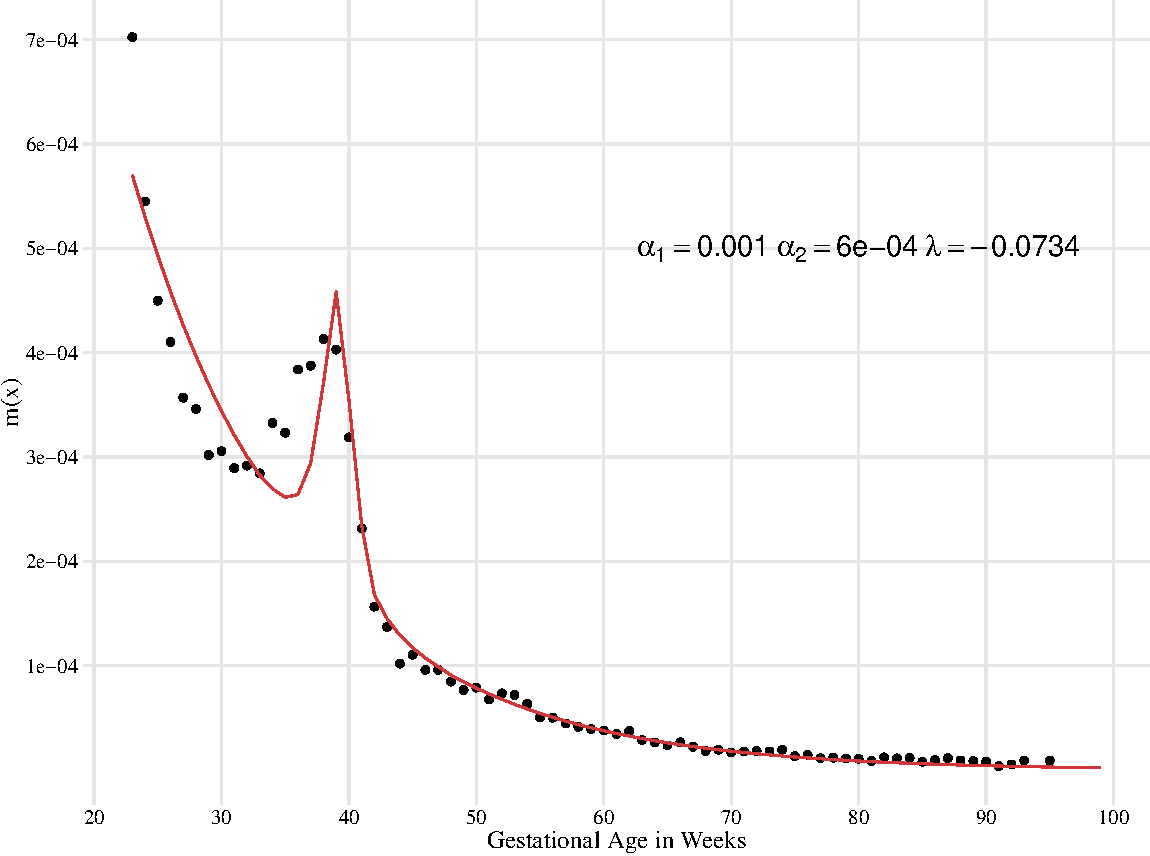
\includegraphics[width = 0.8\textwidth]{./fig/fimort_mx_model1.pdf} \\
Modelling the gestational age pattern of human mortality, US, conception cohort 2009.
\end{figure}

\end{frame}

\begin{frame}
\frametitle{\insertsection}

$\text{f}(b)$ assumed to follow a Beta distribution bound to weeks 23 to 47.

\begin{figure}[htb!]
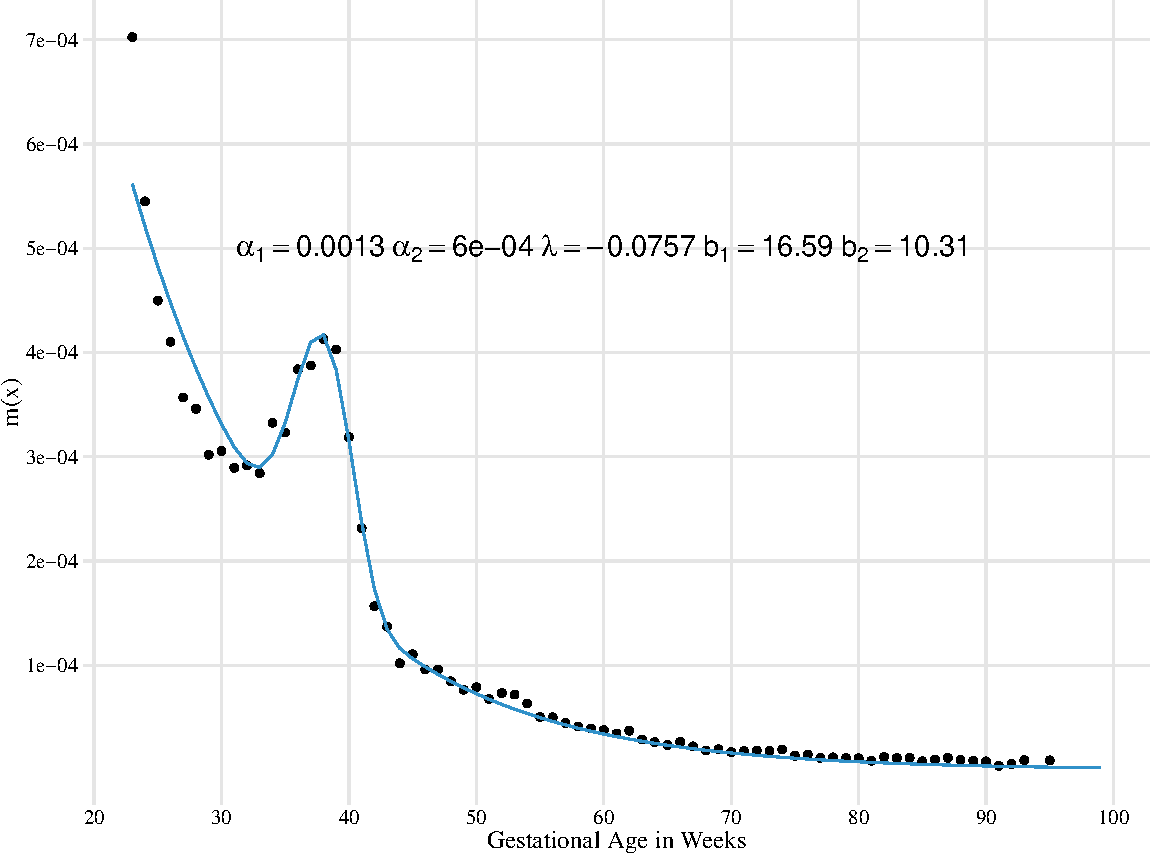
\includegraphics[width = 0.8\textwidth]{./fig/fimort_mx_model2.pdf} \\
Modelling the gestational age pattern of human mortality, US, conception cohort 2009.
\end{figure}

\end{frame}

\section{References} %%%%%%%%%%%%%%%%%%%%%%%%%%%%%%%%%%%%%%%%%%%%%%%%%%%%%%%%%%

\begin{frame}
\frametitle{\insertsection}

  \printbibliography

\end{frame}

\end{document}